\section{Week 1}

\begin{wrapfigure}{tr}{.3\textwidth}
 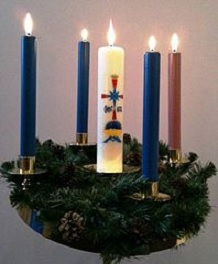
\includegraphics[scale=.6]{x20221125AdventMeditationWeek1-img001.jpg} 
\end{wrapfigure}

Just as we celebrate and
anticipate the Incarnation of the Logos on the material plane, so, too, we want to prepare for the analogous birth
within the human soul.
\textbf{Valentin Tomberg}, in Letter II, refers to the “second birth” as \emph{Christian Yoga}. Hence, the elements of
Christian Yoga are analogous to the stages of yoga described by \textbf{Patanjali} in the \emph{Yoga Sutras}. In Letter
XVI, \emph{The Tower of Destruction}, these stages are related to the three stages of the spiritual life described by
\textbf{St. John of the Cross}. Hence, we have a schema relating these yoga stages in three languages as exposed in Table~\ref{tab:AdvMedWeek2}.

\begin{table}[t]
\centering
\begin{tabular}{*4l}
\toprule
\textbf{Sanskrit} &
\textbf{Greek} &
\textbf{English} &
\textbf{Spiritual Life}\\\midrule
Dharana &
Catharsis &
Concentration &
Purification\\
Dhyana &
Theoria &
Meditation &
Illumination\\
Samadhi &
Theosis &
Contemplation &
Mystical Union\\\bottomrule
\end{tabular}
\caption{\small Stages of Christian Yoga}\label{tab:AdvMedWeek2}
\end{table}

Tomberg contrasts the Vedantic ideal with the Christian goal. The former, he says, leads to the extinction of
consciousness, whereas the Christian goal is the “unity of two”. For more on the differences between Yoga and
Christianity, see \emph{Studies in the Psychology of the Mystics} by \textbf{Joseph Marechal, S.J}\footnote{}, so we
needn't be concerned about that topic at this point.

The Greek Mystic \textbf{Nicholas Cabasilas} in \emph{The Life in Christ }explains that there are three obstacles to
theosis. These are:

\begin{enumerate}
\item \textsc{Nature}. The Divine nature is different from human nature. 
\item \textsc{Sin}. A will corrupted by evil separate us from God. 
\item \textsc{Death}. In the mortal body, we can see only the dim reflection in the mirror; in this state our bodies are
dominated by sense life. 
\end{enumerate}
These obstacles are overcome by the following historical events respectively:

\begin{enumerate}
\item \textsc{Incarnation}. This unites the human and divine natures in one person. 
\item \textsc{Crucifixion}. The leads to the forgiveness of sins. 
\item \textsc{Resurrection}. This overcomes death and the attraction to sense life. 
\end{enumerate}
Cabasilas relates these ideas to the effects of the sacraments, or mysteries, with the aim of salvation. The esoteric
path aims beyond this to liberation. That aim is union while still in the mortal body:

\begin{enumerate}
\item Purify our soul so it becomes the perfect reflector of the Holy Spirit. 
\item Expose our false sense of I, replaced with the mind of Christ. 
\item Move from a life of instinct to a life of intelligence and love. 
\end{enumerate}
The first step is concentration without effort, which depends on detachment and purification (See Letter XVI)

\begin{itemize}
\item \textsc{Detachment }is the separation from “arbitrary, personal activity”. We are no longer absorbed in the
minutiae of life, but are living on a higher level. 
\item \textsc{Purification }is the cleansing of the mirror by no longer being agitated by emotional disturbances, etc. 
\end{itemize}
\begin{quotationx}
Spirit must become divine Breath in place of arbitrary, personal activity, and Water must become a perfect mirror of the
divine Breath instead of being agitated by disturbances of the imagination, passions and personal desires. Reintegrated
consciousness must be born of Water and Spirit, after Water has once again become Virginal and Spirit has once again
become divine Breath or the Holy Spirit. Reintegrated consciousness therefore becomes born within the human soul in a
way analogous to the birth or historical incarnation of the WORD. \flright{\emph{Meditations on the Tarot. Letter II: The High Priestess}}

\end{quotationx}

\flright{\itshape Posted on 2022-11-25 by Cologero}

\begin{center}* * *\end{center}

\begin{footnotesize}\begin{sffamily}
\texttt{Balder on 2022-11-28 at 15:41 said:}

You have almost converted me with Christmas Meditations. It seems I retain many of those things named animistic in the pamphlet and they are impossible to discard. Perhaps I should build upon them.

\hfill

\texttt{rui artur on 2022-11-30 at 08:36 said:}

{@} Balder,

there is nothing in the Christian revelation which is opposed to an animistic conception of reality – in fact, it presupposes it. Except perhaps some specific practices (but even those are liable to be syncretized).

\hfill

\texttt{Balder on 2022-12-01 at 04:14 said:}

Rui Artur, I think you are right. But my worldview is throughly Pagan. Like the old pagan gnostics of old, I can only underwrite some aspects of the Christian dogma, creed and ethics, and also the metaphysics of Christianity because of its theological dimension is bereft of the total and higher significance of Aryan Metaphysics and esotericism, which I think (like Guénon) can be found from the Advaita Vedanta and from the Eastern Metaphysics, and from the Indo-European line. This is why I consider myself as a Gnostic Christo-Pagan. The parts of the Bible I highly value are some of the Torah, and from the New Testament especially the Gospel of John, Sermon on the Mount – which I consider to be the highest ethical teaching given to mankind as counsels of perfection – and the Apocalypse, which I consider to be Hyperborean teachings in origin.

As a person I still consider myself being largely under the impulse of the Finno-Ugric national spirit Lemminkäinen or Kaukomieli, or the Norse Balder, who like Osiris, Jesus and Tammuz and the like live, die, resurrect and live free in the new World in the New Heaven and Earth. The Ragnarök went already.

\hfill

\texttt{Kaukomieli on 2022-12-02 at 06:43 said:}

I must mention that there has been an attempt to synthesize Christianity with the doctrine of Non-Dualism of the Vedanta. The book is called Christianity and the Doctrine of Non-Dualism, the writer “A Monk of the West”. It was quite a baffling reading I must admit.

\url{https://www.sophiaperennis.com/books/christianity/christianity-and-the-doctrine-of-non-dualism/}

\hfill

\texttt{Arthur Konrad on 2022-12-02 at 08:10 said:}

Perennialism implies a belief that certain traditions contain teachings which have objective value, and that these traditions partially overlap, or overlap on important points (and on others they don’t). Therefore, to derive value from, or acknowledge the validity of a certain tradition is a matter of practicality, for people who approach this in a practical way. It is easy to see why going an inch further from this can lead to all sorts of extravagances, such as the Perennial Philosophy, Traditionalism, New Ageism, etc. This is of course, all very Western.

So, what is the practical value of having a ‘Pagan worldview’ nowadays? I’m asking this honestly. For it somehow applies that one has it, and another does not, so what in it is distinctly Pagan which is not in fact, in its positive aspects, merely Universal? Doing away with the whole concept of ‘Paganism’ is in my opinion, in the first order a matter of good education – is there anything more absurd than to call the Roman religion a ‘Pagan’ (i.e. ‘rustic’) religion? Or that of Athens or Babylon or Song?

\hfill

\texttt{Kaukomieli on 2022-12-03 at 11:03 said:}

First of all, apologies for Cologero for taking this thread too far afield from the topic. I’ll try to be as short as possible in my answer to Arthur.

{@} Arthur Konrad, of course the term Pagan (or Heathen) is a controversial and not a very good one in that. I have, however, used the term to refer spiritualities of a non-abrahamic kind. In short, your message implies that practicality and utility trumps over idealism and truth. If you’re a pragmaticist and a utilitarian, go and choose to be an trans-sexual Atheist bright, I’m sure you’ll be more welcomed in today’s world than a Christian or a Pagan who sticks to their guns in the face of the onslaught of modernity.

There are some distinctive features of a Pagan worldview that separate it in its essential aspects from the Judeo-Christian and other revelations of the Abrahamic kind (the question of Monotheism being only one). Ancient Paganism, Hermeticism and Christianity are all essential parts of the Western mystery Tradition, and whatever we think about the first, it still runs in the veins of many, and with the words of Tomberg “one must love the pagan past”. Universality, locality and particularism have all their appropriate places. Christ in this picture is the Corner Stone and the Lapis that the builders forgot and rejected.

\hfill

\texttt{Arthur Konrad on 2022-12-03 at 14:46 said:}

{@} Kaukomieli

‘In short, your message implies that practicality and utility trumps over idealism and truth’

Truth is highly practical and utilitarian

‘There are some distinctive features of a Pagan worldview that separate it in its essential aspects from the Judeo-Christian and other revelations of the Abrahamic kind’

The religion today corresponds very much to the impulses and character of the age. One aspect of our age’s character is the insatiable greed for controversy.

\hfill

\texttt{Kaukomieli on 2022-12-03 at 15:25 said:}

{@} Arthur

“Truth is highly practical and utilitarian”

Then I just might suggest youo go ahead and practice some chaos magic, lets say do the invocation of Bugs Bunny and tell us about the results of that meeting with the Christ Rabbit. Their motto is however, if it works, it’s the truth.

“The religion today corresponds very much to the impulses and character of the age. One aspect of our age’s character is the insatiable greed for controversy.”

With following the impuse of Christ we get to eat that sacred super-wordly bread and to drink that sacred essence of holy water which quenches our thirst eternally and would have made Odin himself happy when hanging on the Yggdrasil for nine days and nights. From the spirit of our Bloodline we are life loving joyous and proud pagans; Christ calls to us to trancendental, heavenly happiness.

\hfill

\texttt{Kaukomieli on 2022-12-03 at 16:21 said:}

Christianity………………………..My views

Monotheism………..Panentheism / Monism / Non duality

Trinitarian Doctrine………..Nine-Fold Valknutr / Odin-Vili-Ve

Animal souls dissolve…….Animal souls transmigrate in the group soul

Only one life…………Transmigration / Re-incarnation (the term is debatable,God / Spirit is the only transmigrant)

A new soul in every birth………Pre-Existence of the Soul

Strickt Patriarchy………Norse / European temple of Priests and Priestesses ( not Woman Priests)

Origin of Mazdaen dualism of Good and Evil……….Indo-European and Nordic-Hyperborean line of non duality

Man as Imago Dei………………..confirmed also

Creationism…………………………Emanationism

God as Person the Consummation………Doctrine of the Absolute

Solar Worship / Strickt Right Hand Path………Synthesis of Solar and Lunar cults (the RHP / LHP)

Tendency to absolutism, fundamentalism, and even totalitarianism……..Plurality and Higher unity of multifaceted viewpoints

Strickt Orthodoxy…………….No Heresy if practical ethics are in line

Judeo-Christian calendar year……….Hermetic Solar Year of Euinoxes and Solstices

Tendency to collectivism…………..Aristocratic Ethics

\hfill

\texttt{Arthur Konrad on 2022-12-03 at 17:29 said:}

I can only assume you verified all these things through personal insight

P.S. What is a Judeo-Christian calendar year?

\hfill

\texttt{Kaukomieli on 2022-12-04 at 19:59 said:}

{@} Arthur

“I can only assume you verified all these things through personal insight”

Yes. I deciphered them from the universal mind.

“What is a Judeo-Christian calendar year?”

I think Cologero is speaking a little about that in this topic.

\hfill

\texttt{Kaukomieli on 2022-12-04 at 20:48 said:}

{@}\! Arthur, cordially and humbly: “Who is among you who gives your brother a stone (the doctrine) if he asks for bread (practical life wisdom)”?

You say: truth is practical and utilitarian. I ask you, is what is practical and useful the truth?

\hfill

\end{sffamily}\end{footnotesize}
